\documentclass[tikz,border=10pt]{standalone}
\usepackage{tikz}
\usetikzlibrary{shapes.geometric, arrows.meta, positioning, calc, fit, backgrounds}
\usepackage{amsmath,amssymb}
\usepackage{xcolor}

% Unified Academic Color Palette
\definecolor{cInput}{RGB}{235, 248, 255}
\definecolor{bInput}{RGB}{49, 130, 206}

\definecolor{cTrans}{RGB}{240, 249, 255}
\definecolor{bTrans}{RGB}{43, 108, 176}

\definecolor{cGCN}{RGB}{230, 255, 250}
\definecolor{bGCN}{RGB}{49, 151, 149}

\definecolor{cRecurr}{RGB}{250, 245, 255}
\definecolor{bRecurr}{RGB}{128, 90, 213}

\definecolor{cHead}{RGB}{255, 245, 245}
\definecolor{bHead}{RGB}{229, 62, 62}

\definecolor{cFusion}{RGB}{254, 252, 191}
\definecolor{bFusion}{RGB}{214, 158, 46}

\definecolor{cGray}{RGB}{247, 250, 252}
\definecolor{bGray}{RGB}{160, 174, 192}

\definecolor{tDark}{RGB}{26, 32, 44}
\definecolor{tMuted}{RGB}{74, 85, 104}

\begin{document}
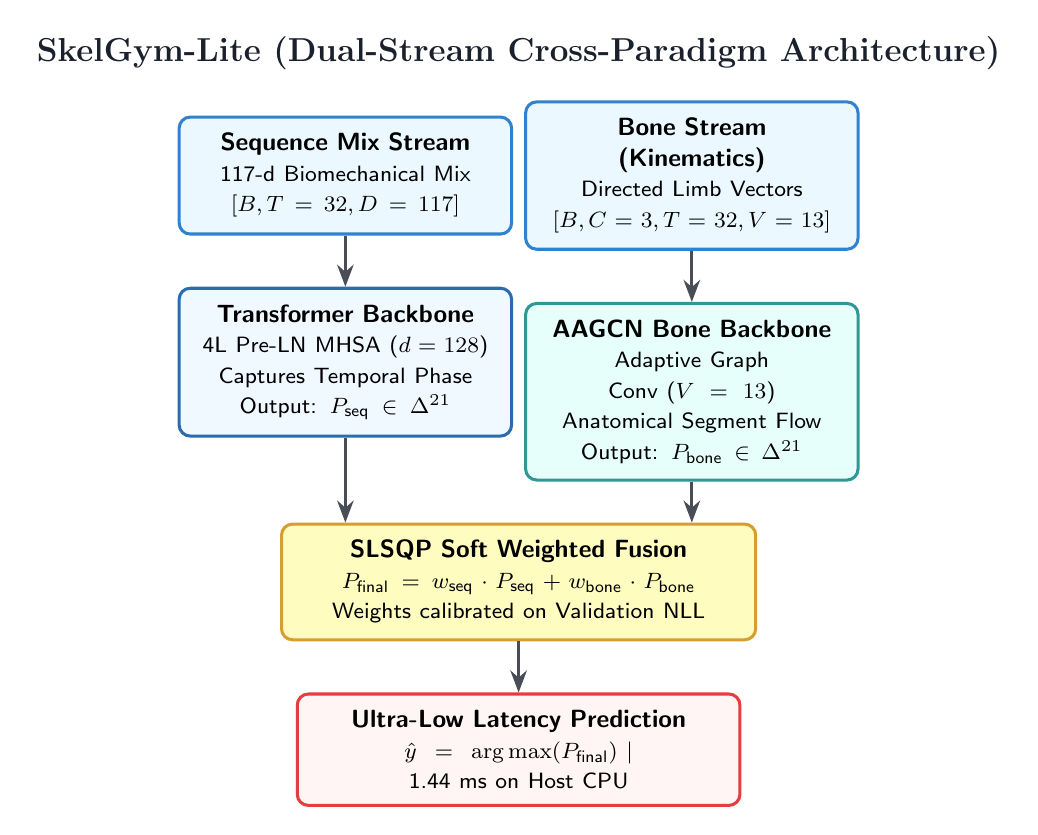
\begin{tikzpicture}[
    font=\sffamily\small,
    >=Stealth,
    node distance=0.65cm,
    block/.style={
        draw=#1,
        line width=1.1pt,
        rounded corners=4pt,
        align=center,
        inner sep=6pt
    },
    arrow/.style={->, line width=1.1pt, color=tDark!80}
]

\node[font=\bfseries\large, text=tDark] (title) at (3.8, 1.55) {SkelGym-Lite (Dual-Stream Cross-Paradigm Architecture)};

% Stream 1: Transformer
\node[block=bInput, fill=cInput, text width=3.8cm] (in1) at (1.6, 0) {
    \textbf{Sequence Mix Stream}\\
    {\footnotesize 117-d Biomechanical Mix}\\
    {\footnotesize $[B, T=32, D=117]$}
};

\node[block=bTrans, fill=cTrans, text width=3.8cm, below=of in1] (back1) {
    \textbf{Transformer Backbone}\\
    {\footnotesize 4L Pre-LN MHSA ($d=128$)}\\
    {\footnotesize Captures Temporal Phase}\\
    {\footnotesize Output: $P_{\text{seq}} \in \Delta^{21}$}
};

% Stream 2: AAGCN Bone
\node[block=bInput, fill=cInput, text width=3.8cm] (in2) at (6.0, 0) {
    \textbf{Bone Stream (Kinematics)}\\
    {\footnotesize Directed Limb Vectors}\\
    {\footnotesize $[B, C=3, T=32, V=13]$}
};

\node[block=bGCN, fill=cGCN, text width=3.8cm, below=of in2] (back2) {
    \textbf{AAGCN Bone Backbone}\\
    {\footnotesize Adaptive Graph Conv ($V=13$)}\\
    {\footnotesize Anatomical Segment Flow}\\
    {\footnotesize Output: $P_{\text{bone}} \in \Delta^{21}$}
};

\draw[arrow] (in1) -- (back1);
\draw[arrow] (in2) -- (back2);

% Fusion
\node[block=bFusion, fill=cFusion, text width=5.6cm, below=0.8cm of $(back1.south)!0.5!(back2.south)$] (fuse) {
    \textbf{SLSQP Soft Weighted Fusion}\\
    {\footnotesize $P_{\text{final}} = w_{\text{seq}} \cdot P_{\text{seq}} + w_{\text{bone}} \cdot P_{\text{bone}}$}\\
    {\footnotesize Weights calibrated on Validation NLL}
};

\node[block=bHead, fill=cHead, text width=5.2cm, below=of fuse] (pred) {
    \textbf{Ultra-Low Latency Prediction}\\
    {\footnotesize $\hat{y} = \arg\max(P_{\text{final}})$ \textbar{} 1.44 ms on Host CPU}
};

\draw[arrow] (back1.south) -- (fuse.north -| back1.south);
\draw[arrow] (back2.south) -- (fuse.north -| back2.south);
\draw[arrow] (fuse) -- (pred);

\end{tikzpicture}
\end{document}
